%%%%%%%%%%%%%%%%%%%%%%%%%%%%%%%%%%%%%%%%%%%%%%%%%%%%%%%%%%%%%%%%%%%%%%%%%%%%%

\chapter{Context historique}

\section{Musique en Russie au début du XIX\ieme{} siècle}

Au début du XIX\ieme{} siècle, la Russie accuse un retard considérable pour ce qui est de la musique instumentale (symphonies, concertos, etc..). Cependant, c'est une période où le pays se transforme profondément. La société devient plus citadine et pratique d'avantage la musique occidentale.

En 1802, la \emph{société philharmonique de Saint Pétersbourg} est crée par des personnalités du monde de la culture, du monde de la finance, des musiciens et de riches aristocrates. La capitale découvre les œuvres peu connues de Mozart, Hayden et Beethoven. C'est ainsi, par exemple, que la \emph{Missa Solemnis} de Beethoven est donnée le 26 mars 1824 soit deux semaines avant la crétion viennoise.

Malgré les guerres napoléoniennes, la culture française demeure très appréciée par la haute société. Il en va de même pour la musique française et l'opéra italien. Rossini est découvert au cours des années 1820 et Verdi au cours des années 1840. Des musiciens tels que John Field (professeur de Mikhaïl Glinka) ou encore Anton Herke (professeur de Piotr Tchaïkovski ou Modeste Moussorgski) se chargeront de diffuser l'œuvres de Chopin ou Liszt. A partir des années 1840, les voyages en Russie s'intensifient avec la venue de Liszt, des époux Schumann, de Berlioz puis Wagner ultérieurement.

\section{Naissance de la musique russe}

À partir de 1783, Saint Pétersbourg se dote de son opéra : le \emph{Théâtre de Pierre}. Celui-ci sera succéssivement modernisé en 1802, 1818 et 1836. Comme la vie musicale s'intensifie, trois autres établissements sont construits : le \emph{Théâtre Alexandrinski} (1832), le \emph{Théâtre Mikhailovski} (1833) et le très célèbre \emph{Théâtre Mariinski} (1833).

Mais c'est avec les compositeurs Mikhaïl Glinka (1804-1857) et Alexandre Dargomyjski (1813-1869) que la Russie entame une nouvelle direction avec le développement d'une musique spécifiquement russe. Pour la première fois, il est fait emploi de matériaux historiques et traditionnels de façon réaliste. Le critique musical moderne Viktor Korchikov résume la situation ainsi : « On ne peut pas imaginer le développement de la culture musicale russe sans [...] les trois opéras : \emph{Ivan Soussanine} (Glinka, 1836), \emph{Rouslan et Ludmila} (Glinka, 1837-1842) et \emph{Le Convive de pierre} (Dargomyjski, 1866-1869) ».

Un autre tournant majeur consiste en la création, en 1858, de la \emph{Société Musicale Russe}. Sous l'impulsion d'Anton Rubinstein et sous le patronage de la grande-duchesse Elena Pavlovna, sa mission est de répendre l'enseignement de la musique classique et contemporaine au sein de l'empire. La \emph{Société Musicale Russe} gagne très rapidement en professionalisme. Avec le soutien du prince Nikolaï Troubetskoï, Nicolaï Rubinstein, le frère de d'Anton Rubinstein et grand ami de Piotr Tchaïkovski, devient président \emph{Société Musicale de Moscou}. La création des concervatoires de Saint Pétersbourg (1862) puis de Moucou (1866) compte parmi les plus grandes réussites. Dés lors, la croissance est fulgurante, la \emph{Société Musicale Russe} s'installe à Kiev (1861), à Kazan (1864), à Kharkov (1871), à Nijni Novgorod (187?), etc... Juste avant la révolution de 1917, date de la dissolution et la \emph{Société Musicale Russe}, une cinquataine de filiales sont disséminées dans tout l'empire. 

\section{Le groupe des cinq}

Les guerres napoléoniennes ont entrainé une prise de conscience nationale et l'émmergeance d'un patriotisme officialisé sous le règne de Nicolas I\ier{} (1825-1855).  Sous Alexandre II (1855-1881) puis Alexandre III (1881-1894), les conditions plus libérales sont optimales pour le développement de la \emph{Société Musicale Russe}, mais aussi pour le développement du fameux \emph{Groupe des Cinq}.

Le \emph{Groupe des Cinq} est le cercle de musiciens plus ou moins autodidactes fédéré par Mili Balakirev (chef d'orchestre empirique, 1837-1910) à partir de 1857. César Cui (ingénieur en fortifications, 1835-1918) et Modeste Moussorgski (officier, 1839-1881) furent les premiers à rejoindre le groupe suivis par Nicolaï Rimski-Korsakov (élève officier de marine, 1844-1908) en 1861 puis enfin Alexandre Borodine (médecin et chimiste, 1833-1887) en 1862.

Le goupe défend l'idéal d'une musique spécifiquement russe (folklore national, orientalisme), sur le modèle de Mikhaïl Glinka, libérée de la tutelle des écoles italienne ou allemande. Il est réfractère aux frères Rubinstein mais promouvoit la musique romantiques moderne (Berlioz, Chopin, Liszt, Schumann) plus novatrice et peu encore diffusée en Russie. En 1868, Piotr Tchaïkovski, qui entretient de bonnes relations avec Mili Balakirev et Nicolaï Rimski-Korsakov, espère devenir le sixième membre du groupe. L'éloignement géographique - Tchaïkovski enseigne au conservatoire de Moscou, le \emph{Groupe des Cinq} est basé à Saint Pétersbourg - et le cosmopolitisme de Tchaïkovski interdiront ce rapprochement. À partir de 1872, la réussite et la « traîtrise » de Rimski-Korsakov, l'échec persistant de Cui et la mort de Moussorgski auront raison du cénacle.

Le \emph{Groupe des Cinq} laisse une production musicale importante\footnote{\emph{Islamey} et \emph{Tamara} pour Balakirev, \emph{Le Prince Igor} et \emph{Dans les steppes de l'Asie centrale} pour Borodine, \emph{Une nuit sur le mont Chauve}, \emph{Boris Godounov} et \emph{Tableaux d'une exposition} pour Moussorgski, \emph{Shéhérazade}, \emph{Capriccio espagnol} et \emph{Le Coq d'or} pour Rimski-Korsakov, ...} et jouit d'une importance de premier ordre dans l'histoire de la musique russe.

Une dizaine d'années après la dissolution du groupe des \emph{Groupe des Cinq}, Balakirev forma un second cercle\footnote{D'autres groupes ont existé, citons par exemple le \emph{cercle Belyayev} de Saint Petersburg entre 1885 et 1908 avec Nikolai Rimsky-Korsakov, Alexander Glazunov, Vladimir Stasov, Anatoly Lyadov, Alexander Ossovsky, Witold Maliszewski, Nikolai Tcherepnin, Nikolay Sokolov, Alexander Winkler, etc... } de musiciens dont le membre le plus éminent sera Sergueï Liapounov. Ce mémoire étant dédié à l'étude de l'œuvres de ce dernier, le rapport entre les deux homme sera plus extensivement discuté dans les chapitres suivants. La figure \ref{frise} récapitule la chronologie des événements depuis la naissance de Mikhaïl Glinka jusqu'à la mort de Sergueï Liapounov.

\begin{figure}[!ht]
  \begin{bigcenter}
    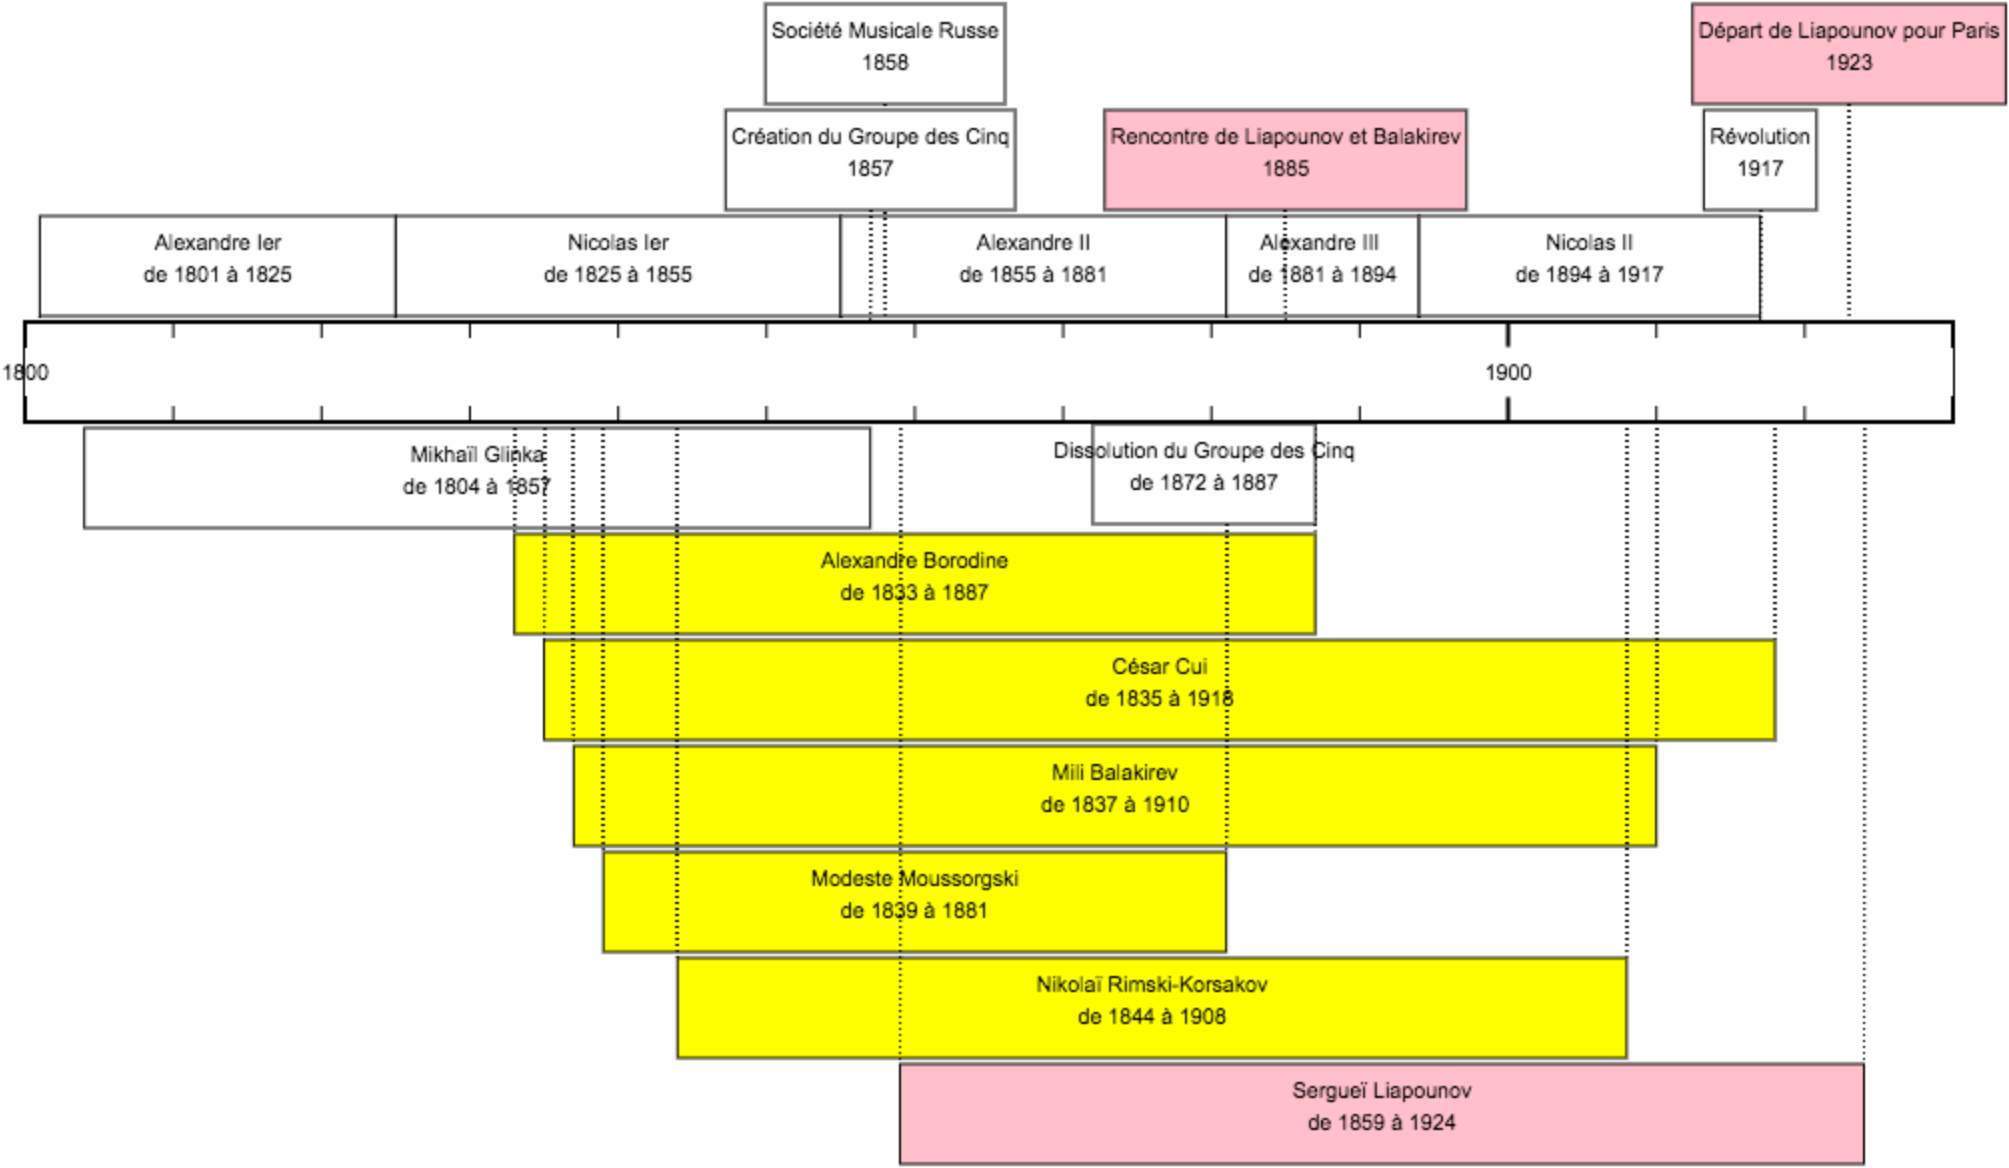
\includegraphics[width=16.0cm, keepaspectratio]{frise.png}
  \end{bigcenter}
  \caption{\label{frise}Frise chronologique des principaux événements depuis la naissance de Mikhaïl Glinka jusqu'à la mort de Sergueï Liapounov.}
\end{figure}

%%%%%%%%%%%%%%%%%%%%%%%%%%%%%%%%%%%%%%%%%%%%%%%%%%%%%%%%%%%%%%%%%%%%%%%%%%%%%
